\documentclass[12pt]{article}
\usepackage[margin=1in]{geometry}
\usepackage{graphicx}
\usepackage{booktabs}
\usepackage{amsmath}
\usepackage{amssymb}
\usepackage{float}
\usepackage{caption}
\usepackage{setspace}
\usepackage[most]{tcolorbox}
\captionsetup{font=small, labelfont=bf, skip=6pt}
\onehalfspacing

\newtcolorbox{explain}{%
  colback=black!3,
  colframe=black!25,
  boxrule=0.5pt,
  arc=1pt,
  left=8pt,
  right=8pt,
  top=5pt,
  bottom=5pt,
  before skip=6pt,
  after skip=12pt,
  fontupper=\normalsize
}

\title{Exploratory Data Analysis\\[0.2em]
\large Bitcoin realized volatility}
\author{Volatility forecasting project}
\date{28 September 2026}

\begin{document}
\maketitle

\noindent
Binance \texttt{BTC/USDT}. Complete UTC days only (24 valid hourly log returns; no gap fill).
Full sample: 3{,}298 days from 18 August 2017 to 26 September 2026.
Time-series plots use 1 January 2025 through the last complete day.
Histograms, moments, ACF/PACF, and ADF tests use the full sample.

\section{Closing price and volume}
\begin{figure}[H]
\centering
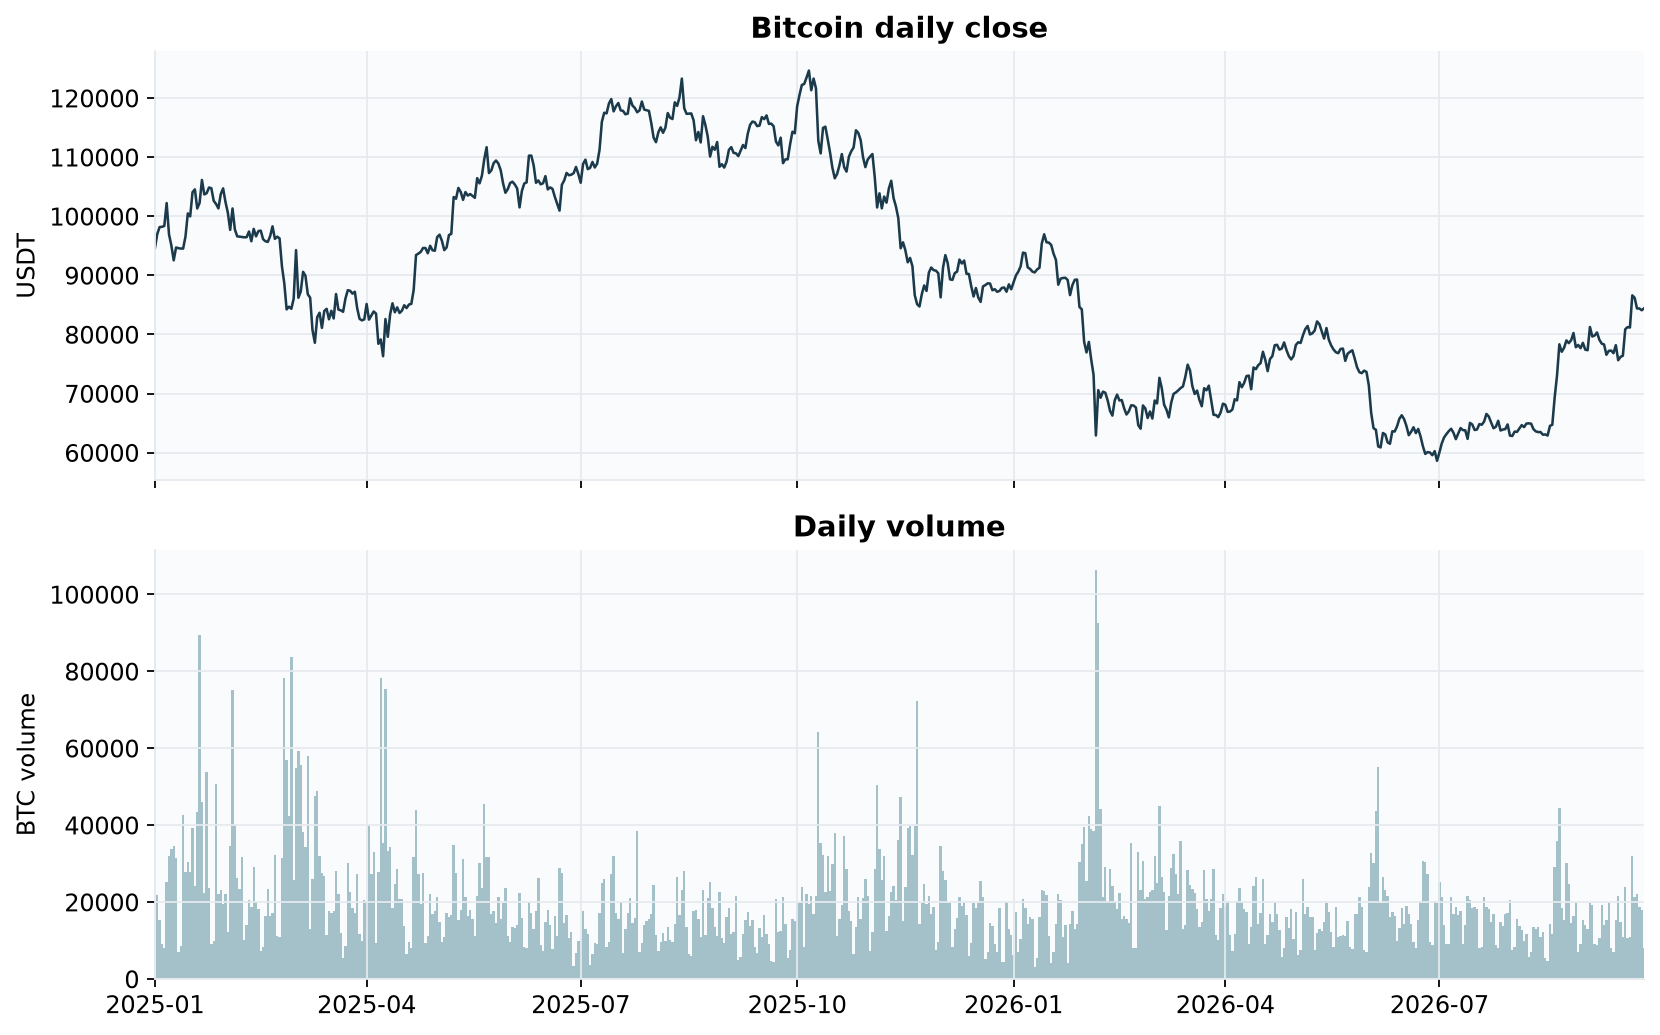
\includegraphics[width=\textwidth]{figures/price_volume.png}
\caption{Daily closing price and trading volume.}
\end{figure}
\begin{explain}
Price and volume set the market context for the volatility series. Volume spikes often line up with sharp price moves, which is consistent with activity concentrating in turbulent episodes rather than arriving uniformly.
\end{explain}

\section{Volume \(z\)-score}
\[
Z^{(30)}_t=\frac{V_t-\mu^{(30)}_t}{\sigma^{(30)}_t}.
\]
\begin{figure}[H]
\centering
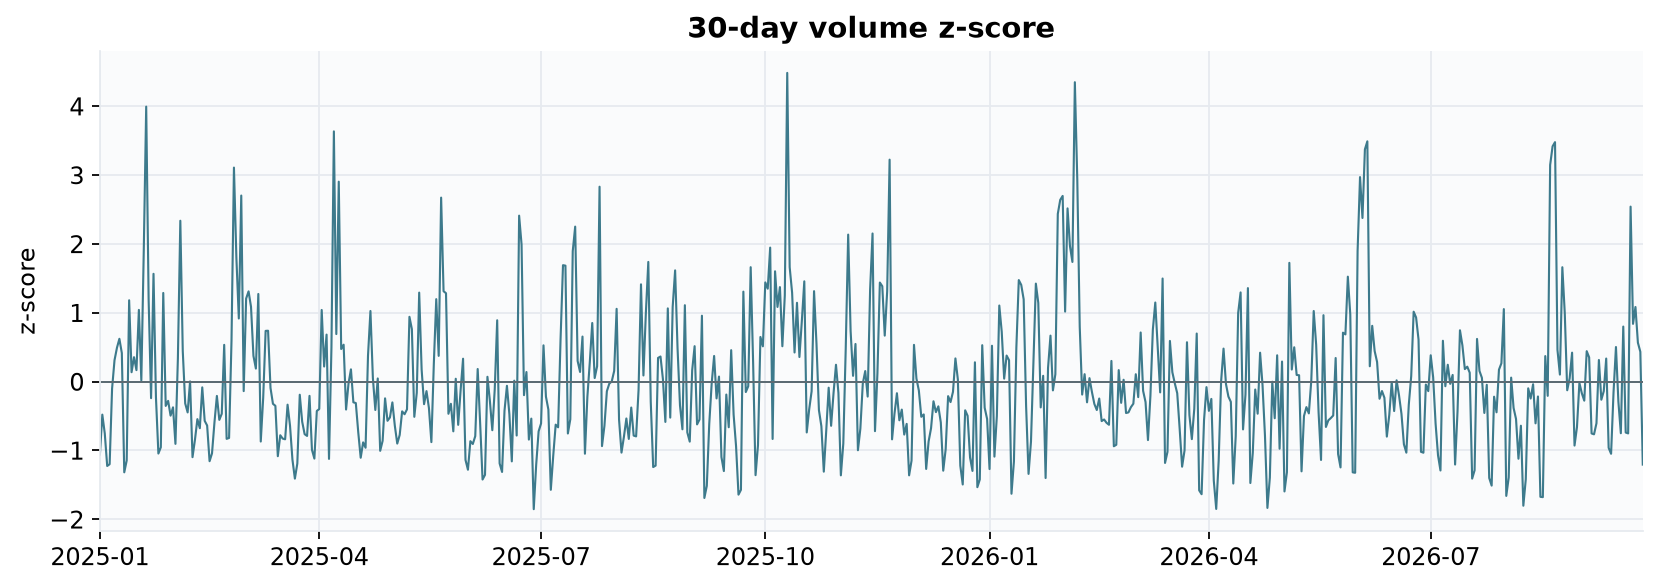
\includegraphics[width=\textwidth]{figures/volume_z.png}
\caption{30-day volume \(z\)-score.}
\end{figure}
\begin{explain}
Large \(|z|\) flags days that are unusually busy or quiet relative to the recent month. Such activity shocks often accompany volatility bursts and are a natural candidate covariate alongside lagged \(\mathrm{RV}\).
\end{explain}

\section{Logarithmic returns}
\[
r_{t,i}=\ln\Bigl(\frac{P_{t,i}}{P_{t,i-1}}\Bigr),
\qquad
R_t=\sum_{i\in t} r_{t,i}.
\]
\begin{figure}[H]
\centering
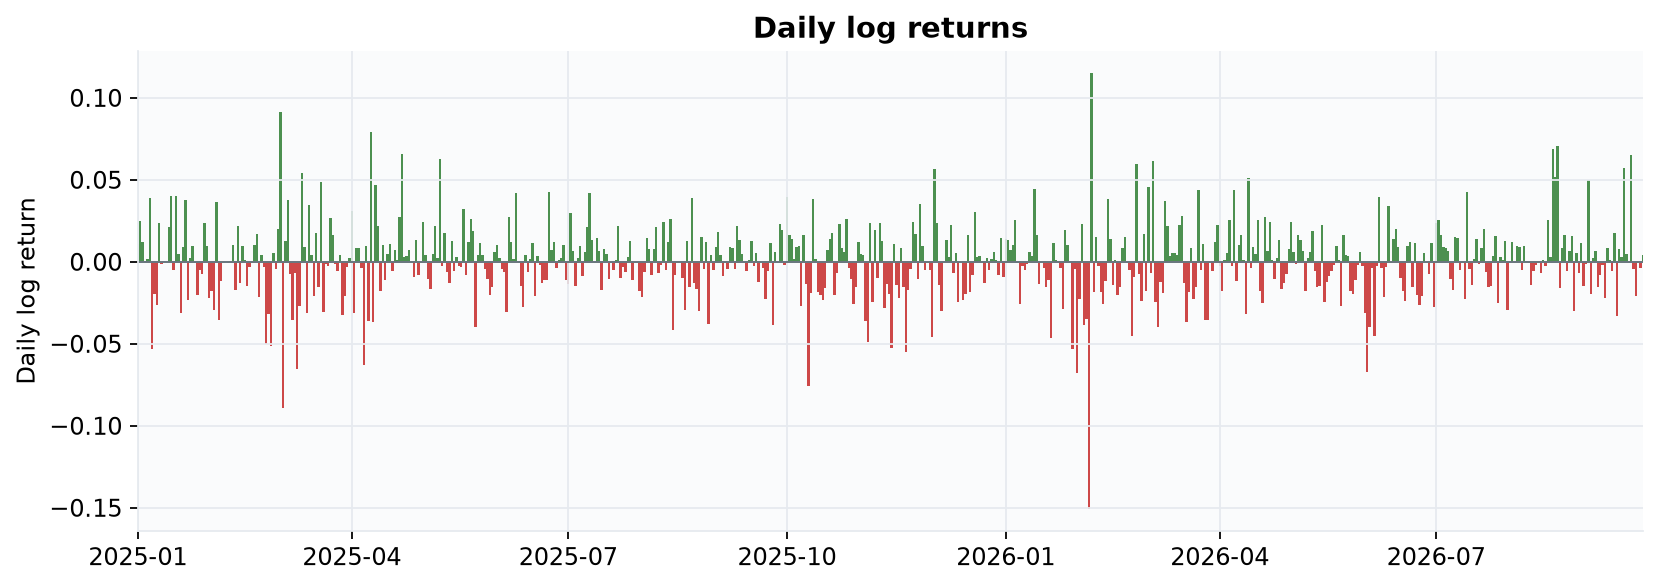
\includegraphics[width=\textwidth]{figures/daily_log_returns.png}
\caption{Daily log returns.}
\end{figure}
\begin{explain}
Daily returns oscillate around zero with frequent large moves of both signs. The path is noisy and only weakly predictable from its own lags; the interesting structure lives in the size of those moves---volatility---rather than in the sign of \(R_t\).
\end{explain}

\section{Distribution of logarithmic returns}
\begin{figure}[H]
\centering
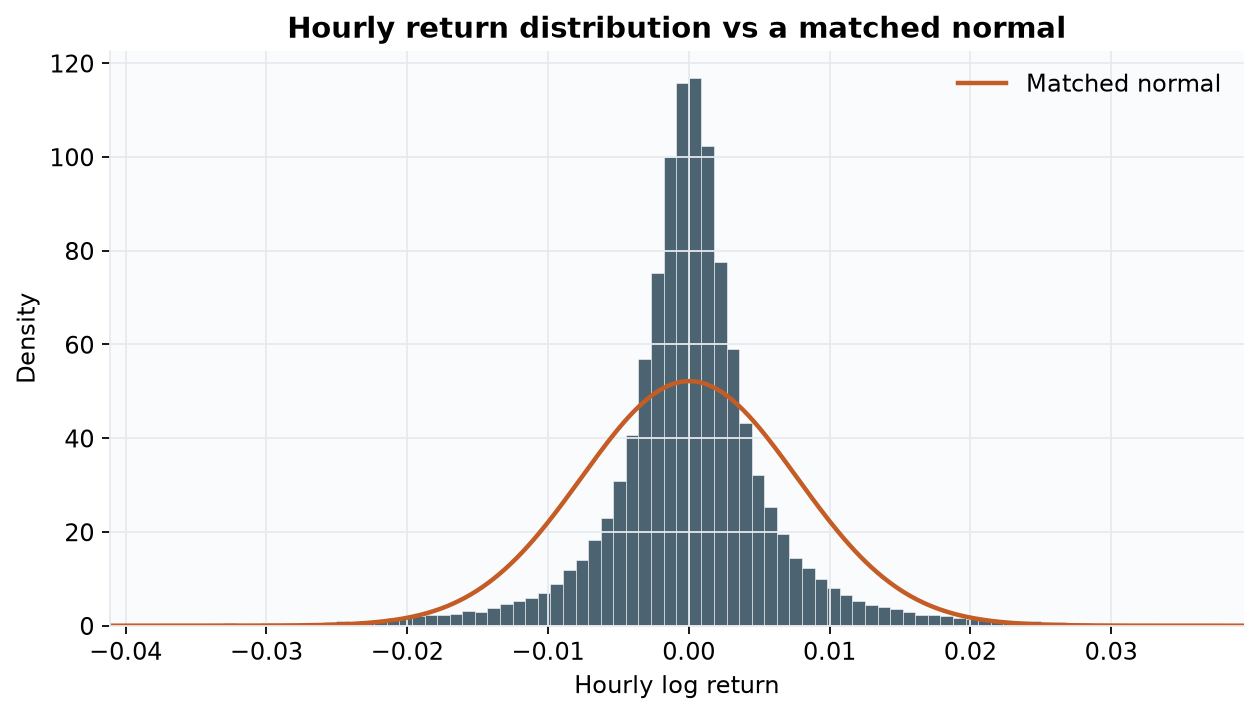
\includegraphics[width=0.92\textwidth]{figures/return_hist.png}
\caption{Distribution of hourly log returns versus a matched normal.}
\end{figure}
\begin{explain}
Hourly log returns---the building blocks of \(\mathrm{RV}_t\)---are heavy-tailed relative to a matched normal (skewness about \(-0.47\), excess kurtosis about \(37\)). Large gains and losses are far more common than Gaussian theory allows. The time-series and ACF panels use daily returns for readability; the histogram keeps the hourly grain because aggregation is not needed for a density plot.
\end{explain}

\section{Autocorrelation of logarithmic returns}
ACF and PACF are shown with lag~0 equal to 1 and vertical axis on \([-1,1]\). The shaded band is \(\pm 1.96/\sqrt{n}\approx\pm 0.034\).
\begin{figure}[H]
\centering
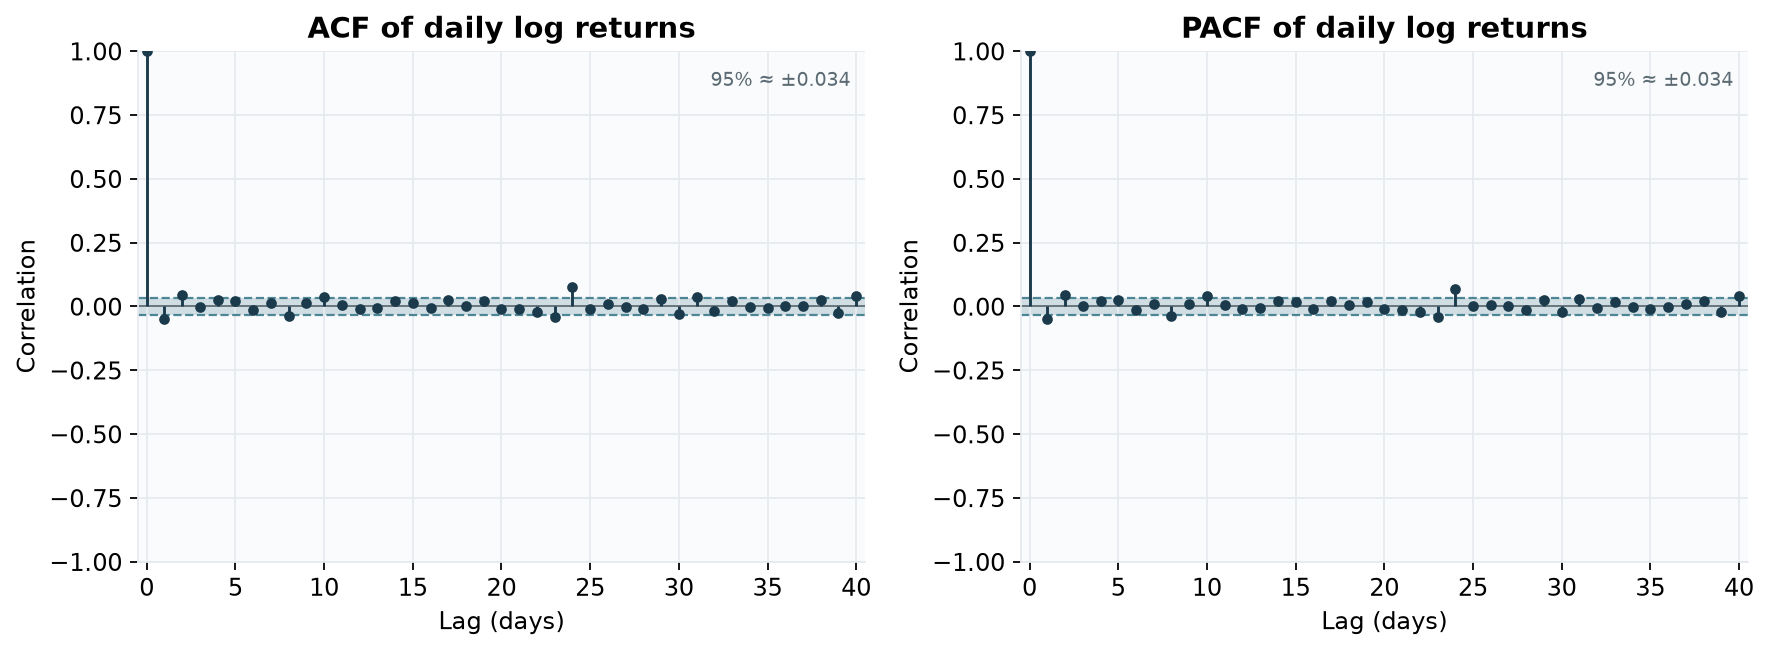
\includegraphics[width=\textwidth]{figures/acf_pacf_returns.png}
\caption{ACF and PACF of daily log returns.}
\end{figure}
\begin{explain}
After lag~0, autocorrelations are small. An ADF test rejects a unit root (statistic \(-11.07\), \(p\approx 4.6\times 10^{-20}\)): returns look stationary and only weakly dependent. The forecasting problem sits in volatility, not in predicting \(R_t\) from its own lags.
\end{explain}

\section{Rolling skewness and kurtosis}
\[
\mathrm{Skew}_t
=
\frac{\mathbb{E}[(r-\bar r)^3]}
{(\mathbb{E}[(r-\bar r)^2])^{3/2}},
\qquad
\mathrm{Kurt}_t
=
\frac{\mathbb{E}[(r-\bar r)^4]}
{(\mathbb{E}[(r-\bar r)^2])^{2}}-3,
\]
computed over the last 30 days of hourly returns.
\begin{figure}[H]
\centering
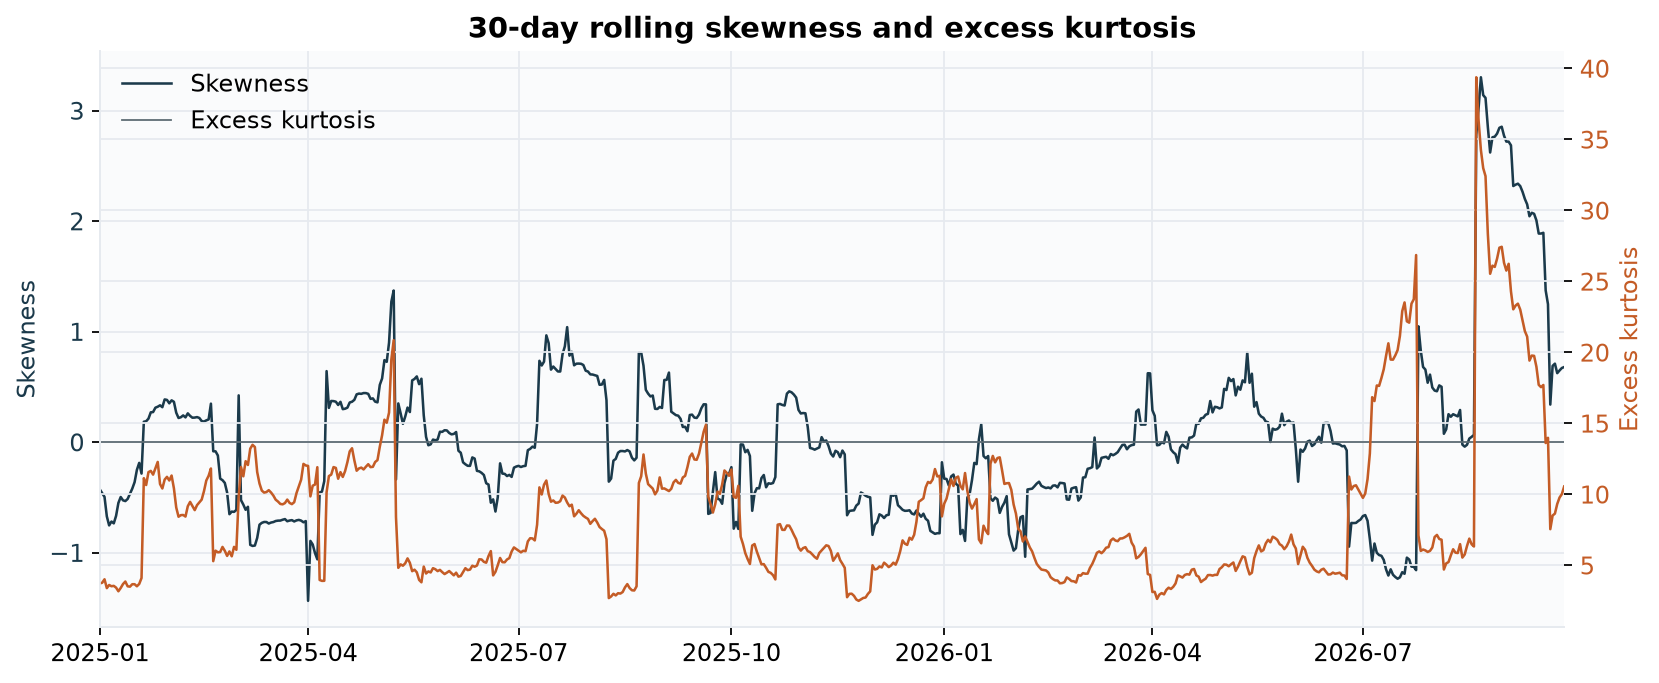
\includegraphics[width=\textwidth]{figures/rolling_skew_kurt.png}
\caption{Rolling 30-day skewness and excess kurtosis of log returns (excess kurtosis $= $ kurtosis $-3$).}
\end{figure}
\begin{explain}
Spikes in excess kurtosis mark windows where extreme moves dominate; those episodes often coincide with high \(\mathrm{RV}\). Skewness shifts show whether recent extremes sit more on the downside or the upside. The two series use different vertical scales.
\end{explain}

\section{Realized volatility}
\[
\mathrm{RV}_t=\sqrt{\sum_{i\in t} r_{t,i}^2},
\qquad
\mathrm{RV}_t^{\mathrm{ann}}=\mathrm{RV}_t\sqrt{365}.
\]
\begin{figure}[H]
\centering
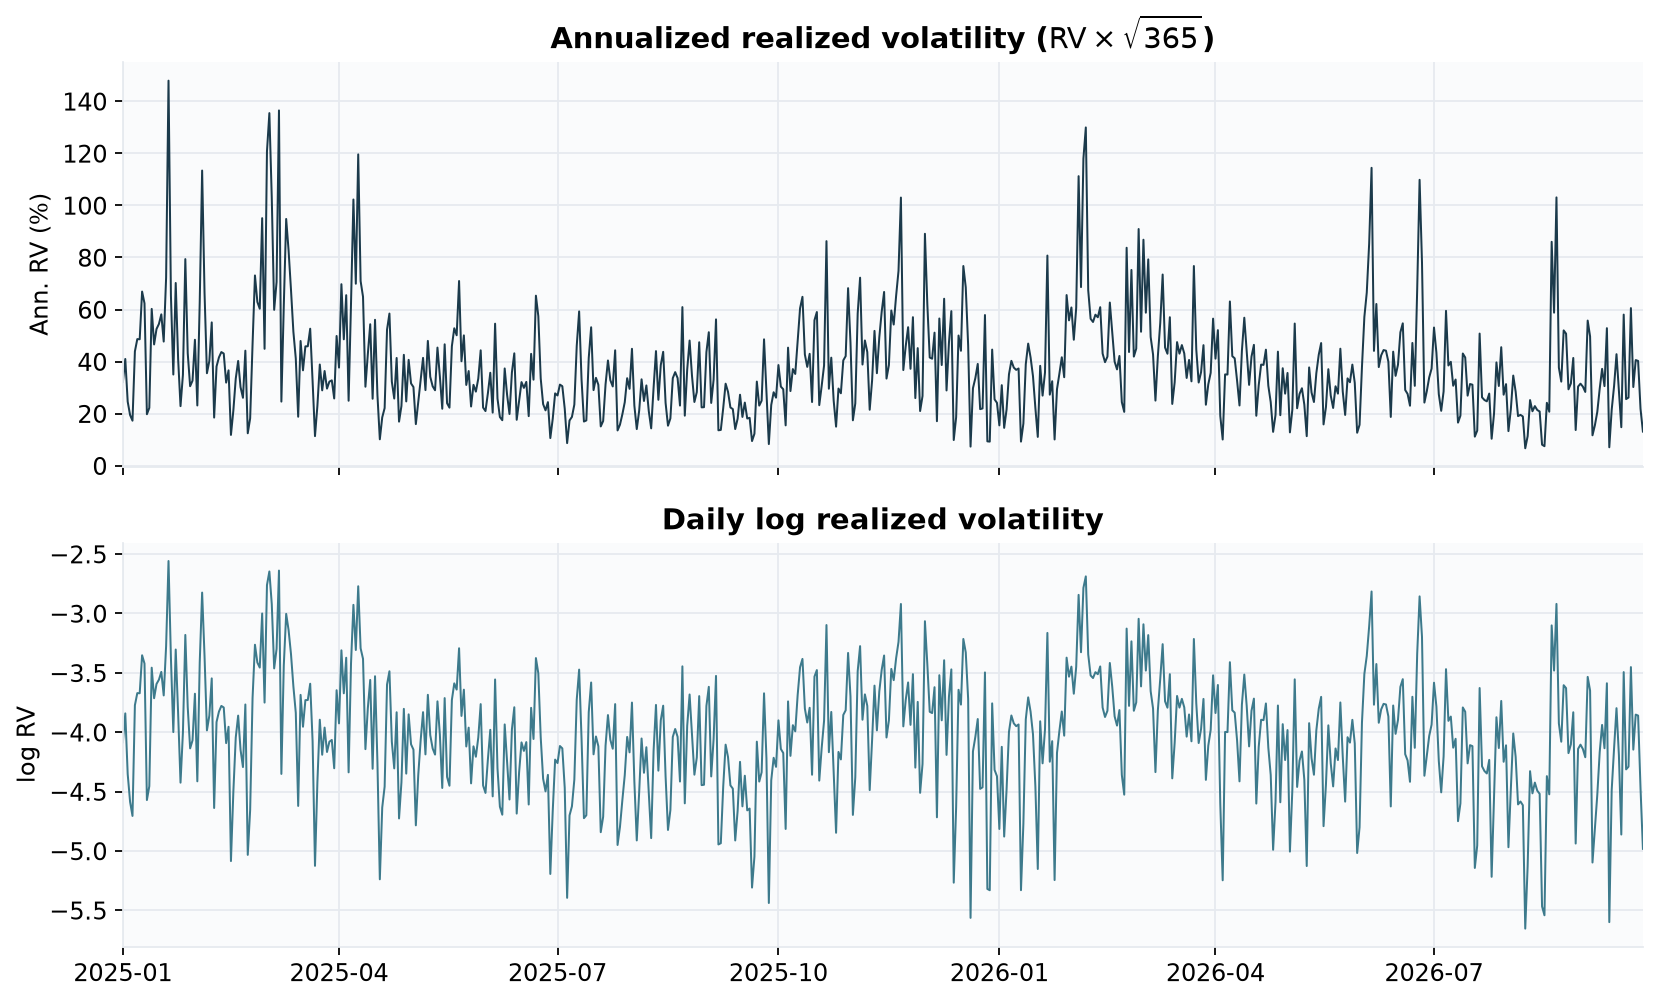
\includegraphics[width=\textwidth]{figures/rv_timeseries.png}
\caption{Annualized daily realized volatility (\%) and \(\log\mathrm{RV}\).}
\end{figure}
\begin{explain}
High- and low-volatility stretches arrive in runs (clustering). The top panel is annualized so the level is readable as a yearly scale (\(100\times\mathrm{RV}\sqrt{365}\) percent); the bottom panel is \(\log\mathrm{RV}\), the smoother scale used for modeling. Full-sample mean annualized RV is about \(57\%\).
\end{explain}

\section{Distribution of RV and \(\log\mathrm{RV}\)}
\begin{figure}[H]
\centering
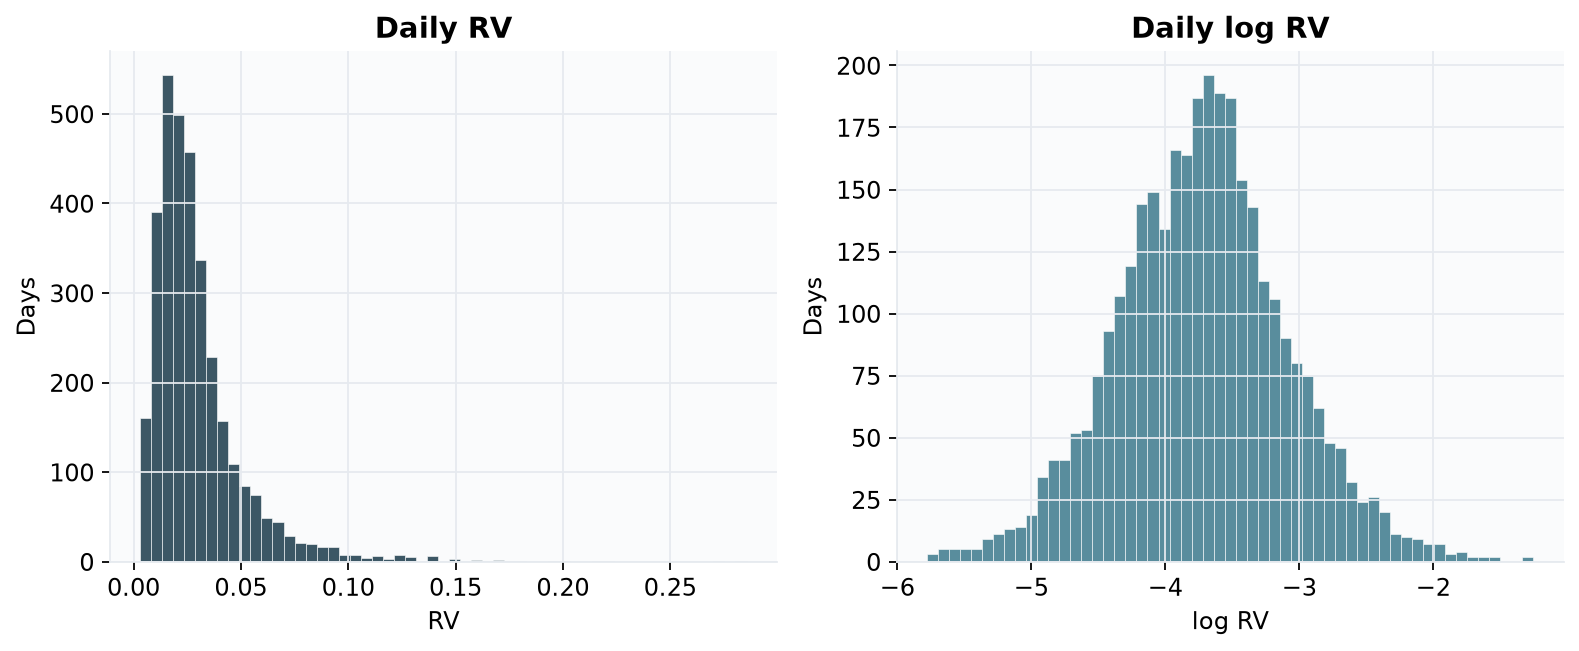
\includegraphics[width=\textwidth]{figures/rv_hist.png}
\caption{Histograms of daily RV and of \(\log\mathrm{RV}\).}
\end{figure}
\begin{explain}
Raw RV is strongly right-skewed (skewness \(3.21\)). \(\log\mathrm{RV}\) is nearly symmetric (skewness \(0.08\), excess kurtosis \(0.36\)), which is a better scale for MSE-type losses and for linear or neural predictors of next-day volatility.
\end{explain}

\section{Autocorrelation of \(\log\mathrm{RV}\)}
\begin{figure}[H]
\centering
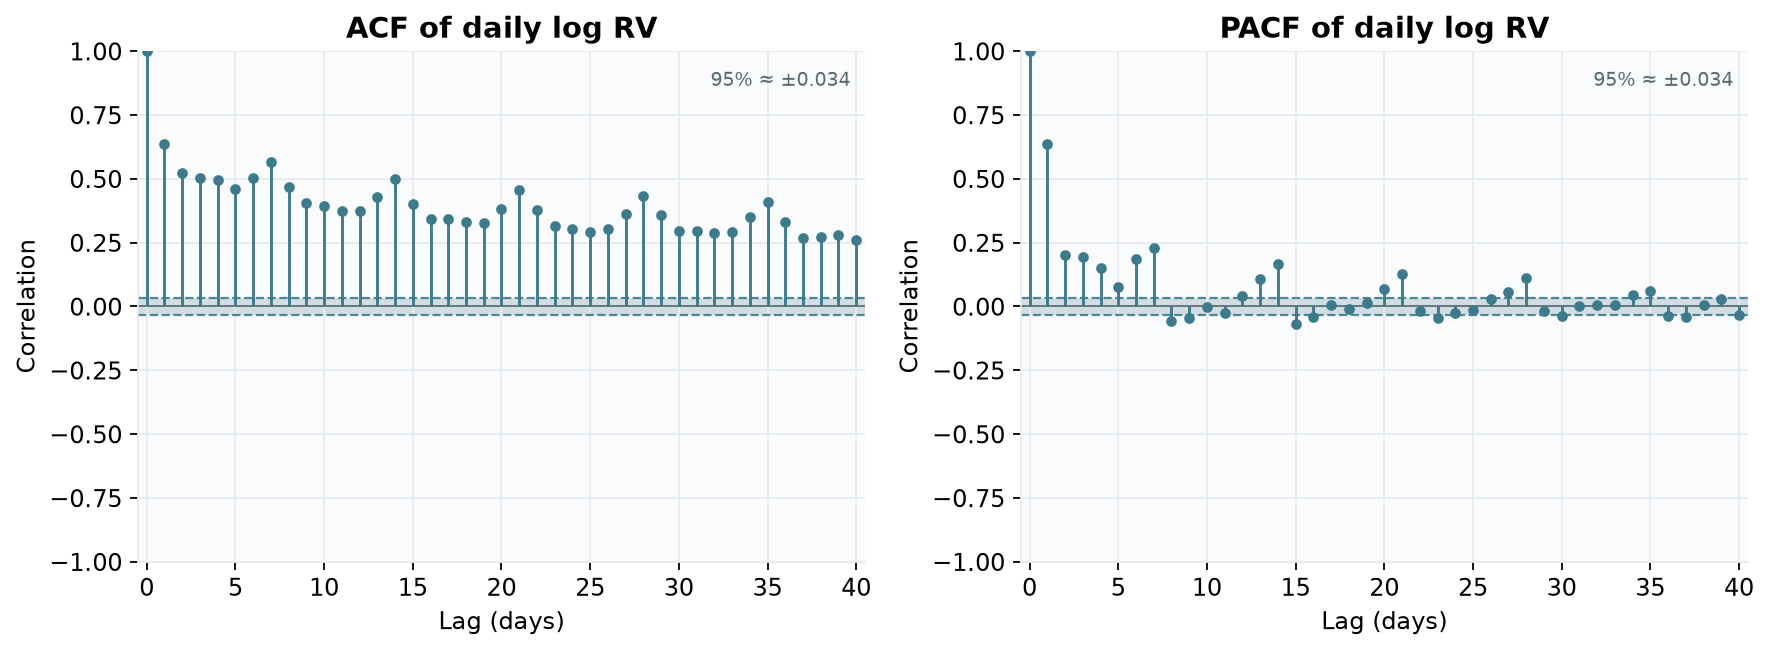
\includegraphics[width=\textwidth]{figures/acf_pacf_log_rv.png}
\caption{ACF and PACF of daily \(\log\mathrm{RV}\).}
\end{figure}
\begin{explain}
The autocorrelation decays slowly (about \(0.63\) at lag~1, \(0.46\) at lag~5, \(0.38\) at lag~22). An ADF test still rejects a unit root (statistic \(-4.86\), \(p=4.2\times 10^{-5}\)): \(\log\mathrm{RV}\) is persistent but stationary. That persistence is the main forecasting signal.
\end{explain}

\section{Relative Strength Index}
\[
\mathrm{RSI}_t=100-\frac{100}{1+\mathrm{RS}_t},
\qquad
\mathrm{RS}_t=\frac{\text{average gain}}{\text{average loss}}
\quad(14\text{ days}).
\]
\begin{figure}[H]
\centering
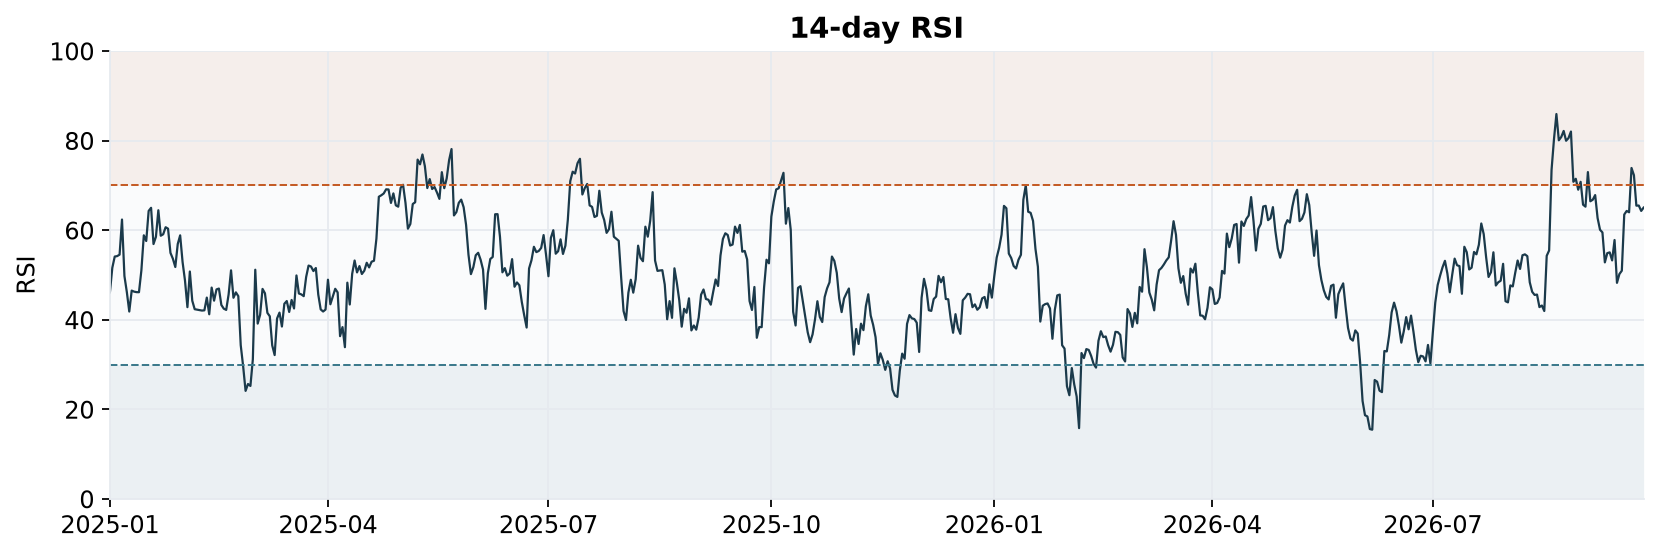
\includegraphics[width=\textwidth]{figures/rsi.png}
\caption{14-day RSI.}
\end{figure}
\begin{explain}
RSI summarizes recent up versus down momentum. Readings above 70 and below 30 mark stretches that are strong relative to the last two weeks; here it is descriptive context, not a volatility forecast by itself.
\end{explain}

\section{Bollinger bands}
\[
\mathrm{Upper}_t=\mathrm{MA}^{(20)}_t+2\,\sigma^{(20)}_t,
\qquad
\mathrm{Lower}_t=\mathrm{MA}^{(20)}_t-2\,\sigma^{(20)}_t.
\]
\begin{figure}[H]
\centering
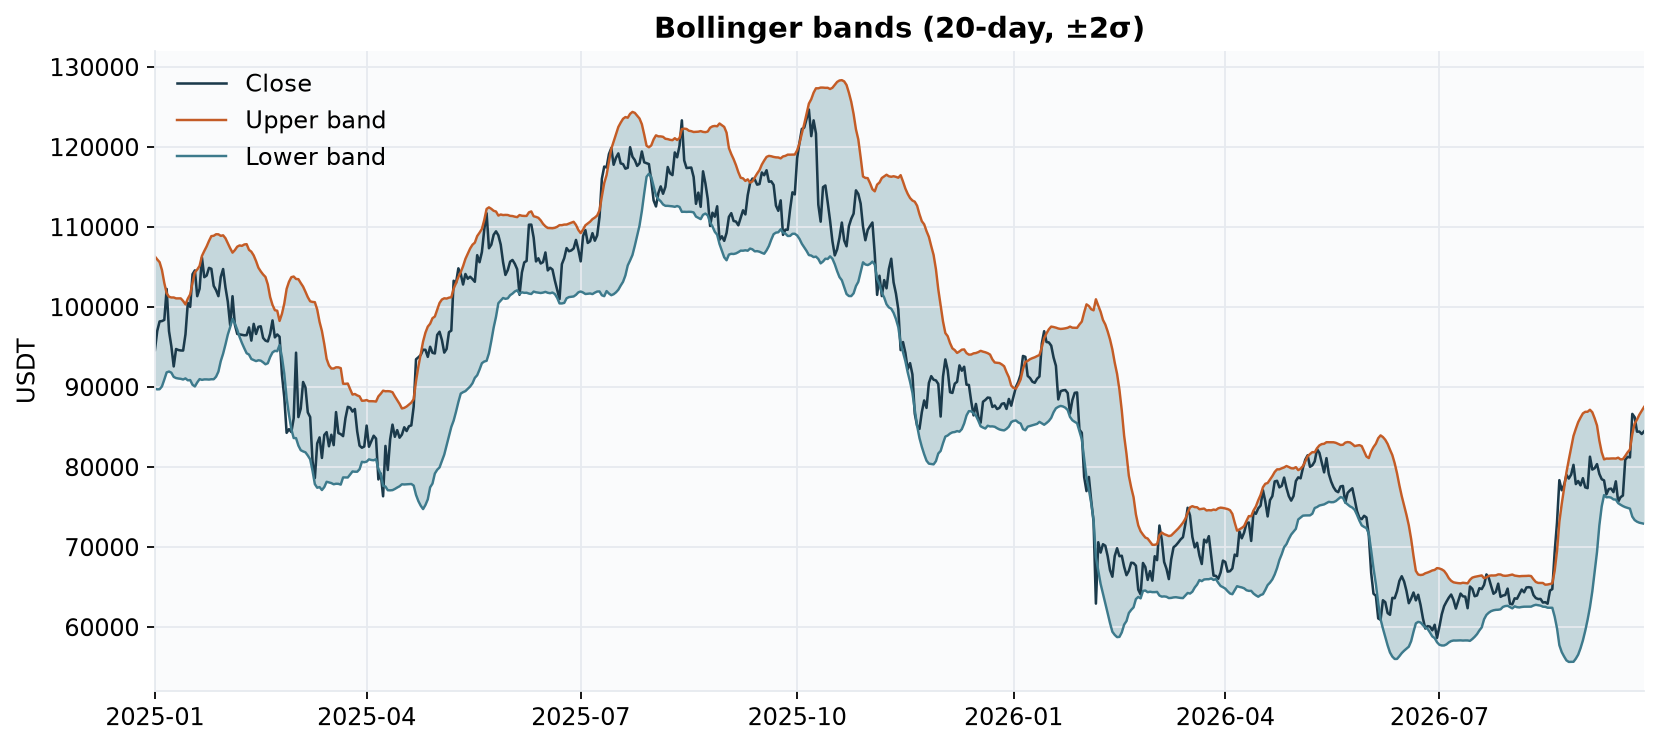
\includegraphics[width=\textwidth]{figures/bollinger.png}
\caption{Closing price with 20-day Bollinger bands (\(\pm 2\sigma\)).}
\end{figure}
\begin{explain}
Band width is a rolling measure of local price dispersion: it widens in turbulent stretches and contracts in calm ones. Touches of the bands locate comparatively stretched prices within the recent 20-day window.
\end{explain}

\section{Synthesis}
Bitcoin returns are weakly autocorrelated and heavy-tailed. Daily realized volatility clusters and \(\log\mathrm{RV}\) is strongly persistent. The log transform removes the strong right skew of raw RV.

These facts support predicting one-day-ahead \(\log\mathrm{RV}\): econometric baselines on lagged volatility and GARCH-family models on returns, then LSTM/GRU under the same chronological out-of-sample protocol (RMSE, MAE, QLIKE).

\end{document}
